
\subsection{Supervised Learning}
\label{sec:supervised_learning}

Supervised learning can be generally thought of as function approximation where, given a set of inputs and expected outputs, a function from the input to the output is approximated by using a set of learning rules. This approximated function is then used to predict the output of some unseen input.


\begin{gather*}
  f(x) = y \xrightarrow[learning]{supervised} f^*(x)=y \\
  \text{$f^*$ is an approximates function of $f$ that is learned by only having access to $x$ and $y$.}
\end{gather*}
The input and output spaces of $x$ and $y$ can be either categorical or continuous. Categorical data can be of the label form, such as True/False, or simply a finite set of keywords. In the categorical space, there are no inequality relationship between categories, meaning that no one category can be said to be "greater than" or "less than" the other, something that \textit{can} be said of the space of continuous numbers (e.g. one can say $2>1$, but one can not say "green" > "white"). This distinction proves to be important later on when considering how to create mathematical models that can correctly 'learn'. For the cases when the input and output space is categorical, the learning process is commonly referred to as \textit{label classification}, an for cases when these input spaces are continuous, learning is called \textit{regression}. We will first address label classification, going over four main models---Perceptron, Neural Networks, Decision Trees, and Regression---and it will be clear why a different approach is required for continuous spaces.
%todo: mention the importance of (lack of) inequality in categorical dataspace.

\subsubsection{Perceptron}
\label{sec:perceptron}
The simplest form of label classification is often referred to as binary classification, in which the classifier (machine learning algorithm) has to discriminate between two classes. For example, a simple binary classification problem would be to discriminate between sets of points on a Cartesian plane (Fig. \ref{fig:two_classes_example}).

\begin{figure}[!h]
  \centering
  \begin{subfigure}{.49\textwidth}
    \centering
    \includegraphics[width=\linewidth]{figures/twoClasses_separable.pdf}
  \end{subfigure} %
  \begin{subfigure}{0.49\textwidth}
    \centering
    \includegraphics[width=\linewidth]{figures/twoClasses_non_separable.pdf}
  \end{subfigure}
  \caption{Two sets of data, one of which is linearly separable (Left) and the other is non linearly separable (Right). Linear separability means that a line can be found that can perfectly segregate the two classes into two sections. A diagonal, horizontal, or vertical line between the blue and red points can be drawn on the left that achieves that goal. However, on the right there is no one line that can be used to separate the red from blue points. This problem of finding a line of separation between two linearly separable data sets can be solved by using a binary classifier, the earliest example of which is the perceptron.}
  \label{fig:two_classes_example}
\end{figure}

 The perceptron was the first machine learning algorithm designed to solve binary classification in linearly separable conditions. Perceptrons were designed to mimic the McCollough-Pitts neuron model which relied on three main components: inputs, weights, and an activation function. In addition to these components, the perceptron had a learning rule that allowed it to learn when to and not to fire. Listing all the components of a perceptron:
\begin{itemize}
  \item \textbf{Inputs}: A dataset of $n$ dimensional points. Each input point $x$ consists of $n$ features such that each input point can be describes as $(x_1, x_2, \dots, x_n)$.
  \item \textbf{Weights}: $n$ weights described as $w_1, w_2, \dots, w_n$. These weights are randomly initialized.
  \item \textbf{Activation function}: a function on which the neuron decides to fire or not fire. The first one was the threshold (or step) function where the neuron fires if the weighted sum of inputs and weights is larger than threshold $\theta$, and doesn't fire otherwise.
  \item \textbf{Learning Rule}: A rule by which the weights change, described below.
\end{itemize}

% After being trained, the perceptron would fire to indicat that it has seen one class of data points (+1) and would not fire to indicate that it has seen the other class of data points (-1). 

A perceptron can be trained by passing to it each data point from the the dataset. In our example (Fig. \ref{fig:two_classes_example}), each data point would have a two-dimensional input consisting of the $x_1$ and $x_2$ values. Since we are working with two dimensions, the perceptron would have two weights $w_1$ and $w_2$. Every time the perceptron encounters a data point it tries to make a prediction by calculating the weighted sum of the inputs $S$  as $\sum_{i=1}^n w_ix_i$. If $S \geq \theta$ then the neuron fires, meaning it predicts the category to be $+1$. If $S < \theta$, the neuron doesn't fire, predicting the category to be $-1$. Given this determination, the perceptron evaluates its predicted output with the actual output of the data point, then manipulating its weights, completing the learning process of the perceptron on that data point. 

The learning process for input $x$, given a true label $\gamma$ and a threshold $\theta$ is summarized by the following updates:
\begin{align}
  S &= \sum_{i=1}^n w_ix_i > 0  \\
  \kappa &= \begin{cases} 
  \label{eq:piecewise_threshold_function}
    +1 \textrm{ if $S$} > \theta \\
    -1 \textrm{ otherwise} 
  \end{cases} \\
  w_{new} &= w_{old} + (\kappa - \gamma)x.
\end{align}

As can be seen from above, the perceptron learns by changing its weights, as this causes the same input to give a different $S$ which in turn could give a different predicted value $\kappa$. Following this learning rule, it can be proven that the perceptron model converges in finite time to a set of weights that result in a perfect classification for all data points in the dataset. A simple implementation of the perceptron was used to solve the sample datasets presented earlier (Fig \ref{fig:perceptron_solution}).

\begin{figure}[!h]
  \centering
  \begin{subfigure}{.49\textwidth}
    \centering
    \includegraphics[width=\linewidth]{figures/perceptron_solvable.pdf}
  \end{subfigure} %
  \begin{subfigure}{0.49\textwidth}
    \centering
    \includegraphics[width=\linewidth]{figures/perceptron_non_solvable.pdf}
  \end{subfigure}
  \caption{The perceptron model can be used to solve binary classification in linearly separable datasets as in the left image. After training, all points below the shown line of separation would be classified as -1, and all points above the line would be classified as +1. Seemingly, this behavior would correctly extrapolate to unseen data points from a similar distribution. In the case of non linearly separable datasets, the perceptron keeps adjusting its weights but never reaches a solution which correctly classifies all data inputs, meaning the model quits after a set limit of iterations through the dataset. This results in a having a line that clearly does not separate the two classes (Right).}
  \label{fig:perceptron_solution}
\end{figure}

The perceptron model did exceptionally well in solving such binary problems when it was introduced, but its lack of versatility when facing non linearly separable datasets resulted in an echoing cry of concern as to how realistic of a learner it could be. In fact, the scathing criticism that the perceptron model received lead to a 10-year hiatus in research on perceptrons \cite{minsky1969perceptrons}. Researchers who worked on the perceptron and neural network fields published under the umbrellas of  "adaptive signal processing", "pattern recognition", and "biological modeling" \cite{Yadav2015}. Slowly but surely, some loyalists to the neural machine learning perspective worked on enhancements to the perceptron model, leading to breakthroughs that skewed public opinion back in favor of what researchers now call neural networks: a group of perceptrons that are linked together to perform learning on datasets that one perceptron alone couldn't learn. 

\subsubsection{Neural Networks}
\label{sec:neural_networks}
Neural networks were first implemented by linking perceptrons together to attempt to solve problems that a single perceptron seemed unable to solve. While initial attempts did not indicate that this approach yielded a distinctly superior model, three major breakthroughs were integral to the uphill battle that neural network researchers had to fight in order to regain recognition in the machine learning field. The first breakthrough came when scientists put several neurons together in different topologies (Fig \ref{fig:perceptron_layers_example}), calling them a neural network. In a neural network, layers can be defined as a collection of nodes that are fed data from a previous layer, perform a calculation on this data, and pass it to another layer or as a final result.  Although the neural network could approximate more functions, there was no clear way to tune the learning rule from one layer to another. This is when the second and third important ideas came about. The second breakthrough was a realization that choosing a different, continuous activation function (as opposed to the discrete step function) could mean that a derivative could be taken (Fig. \ref{fig:activation_functions}). The third was a method by which the chain rule (from calculus) can be employed on the these derivatives that allows error calculations to be passed down from layer to layer reliably, a method called Back Propagation (Fig. \ref{fig:back_propagation}). Together, these breakthroughs caused a resurgence in the field of neural networks which used perceptrons as their building block. When the activation function changed from a step function, the field moved away from the perceptron naming convention, and used the term \textit{learning units} instead (Fig. \ref{fig:activation_functions}, \ref{fig:perceptron_layers_example}). The name change is also because the learning rule changes with the change of the activation function, which moves the learning unit further away from the initial conceptualization of the perceptron model.


\begin{figure}[!h]
  \centering
  \begin{subfigure}{.49\textwidth}
        \centering
        \includegraphics[width=\linewidth]{figures/stepfunction.pdf}
    \end{subfigure} %
    \begin{subfigure}{0.49\textwidth}
        \centering
        \includegraphics[width=\linewidth]{figures/logisticfunction.pdf}
    \end{subfigure}
  \caption{Different activation functions can be applied to the perceptron model. The simplest and earliest activation function is the step function (Left) which outputs either a $+1$ or $-1$. A disadvantage of the step function is that small changes in the weighted sum ($S$) could cause a large change in the output ($\kappa$). This is solved by the sigmoid activation function (right) which gives a output (between $0$ and $+1$) that is proportional to $\S$ within a given range. When a perceptron implements a sigmoid activation unit, it is referred to as a sigmoid learning unit.}
  \label{fig:activation_functions}
\end{figure}



% Credit to http://tex.stackexchange.com/questions/140782/drawing-a-neural-network-architecture
\begin{figure}[!h]
  \centering
  \begin{subfigure}{0.20\linewidth}
    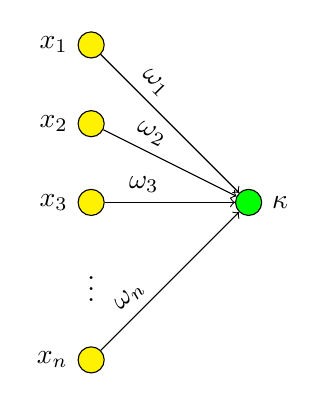
\begin{tikzpicture}
    [   cnode/.style={draw=black,fill=#1,minimum width=3mm,circle},
    ]
        \node[cnode=green,label=0:$\kappa$] (s) at (2,-3) {};
        \node at (0,-4) {$\vdots$};
        % \node at (3,-4) {$\vdots$};
        \foreach \x in {1,...,4}
        {   \pgfmathparse{\x<4 ? \x : "n"}
            \node[cnode=yellow,label=180:$x_{\pgfmathresult}$] (x-\x) at (0,{-\x-div(\x,4)}) {};
            \draw[->] (x-\x) -- node[above,sloped,pos=0.3] {$\omega_{\pgfmathresult}$} (s);
        }
    \end{tikzpicture}
  \end{subfigure}  
  \begin{subfigure}{0.30\linewidth}
  % middle figure
  \centering
  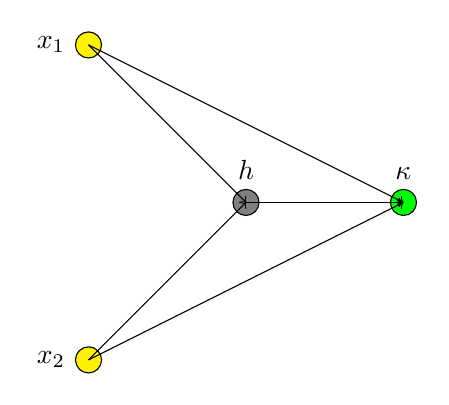
\begin{tikzpicture}
    [   cnode/.style={draw=black,fill=#1,minimum width=3mm,circle},
    ]
        % drwaw the nodes
        \node[cnode=yellow, label=180:$x_1$] (s) at (0,-2) {};
        \node[cnode=yellow, label=180:$x_2$] (s) at (0,-6) {};
        \node[cnode=gray, label=90:$h$] (s) at (2,-4) {};
        \node[cnode=green,label=90:$\kappa$] (s) at (4,-4) {};

        % draw the lines
        \draw[->] (0,-2) -- (2,-4);
        \draw[->] (0,-6) -- (2,-4);
        \draw[->] (0,-2) -- (4,-4);
        \draw[->] (0,-6) -- (4,-4);
        \draw[->] (2,-4) -- (4,-4);
    \end{tikzpicture}
  \end{subfigure}  
  \begin{subfigure}{0.40\linewidth}
    \centering
    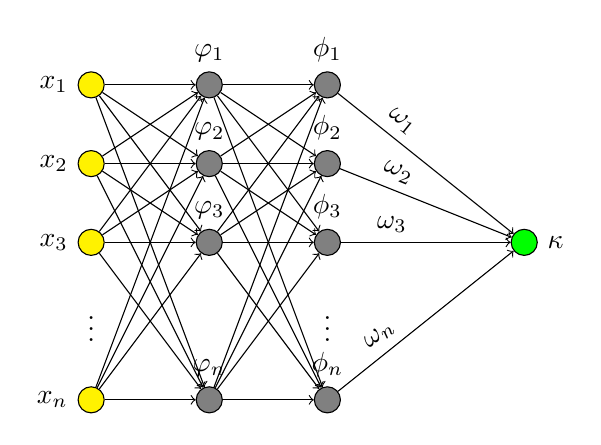
\begin{tikzpicture}
    [   cnode/.style={draw=black,fill=#1,minimum width=3mm,circle},
    ]
        \node[cnode=green,label=0:$\kappa$] (s) at (5.5,-3) {};
        \node at (0,-4) {$\vdots$};
        \node at (3,-4) {$\vdots$};
        \foreach \x in {1,...,4}
        {   \pgfmathparse{\x<4 ? \x : "n"}
            \node[cnode=yellow,label=180:$x_{\pgfmathresult}$] (x-\x) at (0,{-\x-div(\x,4)}) {};
            \node[cnode=gray,label=90:$\varphi_{\pgfmathresult}$] (l-\x) at (1.5,{-\x-div(\x,4)}) {};
            \node[cnode=gray,label=90:$\phi_{\pgfmathresult}$] (p-\x) at (3,{-\x-div(\x,4)}) {};
            \draw[->] (p-\x) -- node[above,sloped,pos=0.3] {$\omega_{\pgfmathresult}$} (s);
        }
        \foreach \x in {1,...,4}
        {   \foreach \y in {1,...,4}
            {   
              \draw[->] (x-\x) -- (l-\y);
              \draw[->] (l-\x) -- (p-\y);
            }
        }
    \end{tikzpicture}
  \end{subfigure}
  \caption{Perceptrons linked in networks with different topologies. Yellow represents input notes, gray represents hidden nodes, and green represents output nodes. The left network contains only one layer, the input layer, with its associated weights that feed into the output layer. This network essentially simulates a computation that is equivalent to the perceptron model. The center network contains a hidden layer composed of simply 1 node. This network can solve the XOR problem, and is able to solve the linearly inseparable dataset in Fig \ref{fig:two_classes_example}. The more nodes added to the hidden layer and the more hidden layers there are, the more communication happens between the nodes in the previous layer, and therefore the higher the abstraction. The network on the right is a more dense network with two hidden layers and many more hidden nodes.}
  \label{fig:perceptron_layers_example}
\end{figure}

A common continuous activation function for learning units is the sigmoid learning unit. Instead of the stepwise function in equation \ref{eq:piecewise_threshold_function}, the output function becomes
\begin{align}
  \kappa &= \sigma(S) = \frac{1}{1+e^{-S}}
\end{align}
which is bounded by 0 and 1. This function is popular because its derivative is rather simple to compute and leads directly into the theory of back propagation. When the sigmoid function is used, the learning rule becomes a minimization of an error term using gradient descent. For a data point with target classification $\lambda$ and predicted classification $\kappa$, the error term is described as
$$ \epsilon = (\lambda- \kappa)^2 $$
and is called MSE and is derived in \ref{sec:regression_supervised_learning}. Gradient descent is an iterative approach to finding the maximum or minimum of a continuous function by using its derivative (Fig. \ref{fig:gradient_descent}).


For example, if a learning unit predicts an output of $\kappa$ with an error $\epsilon$ and it has two learning units feeding it


\begin{align*}
  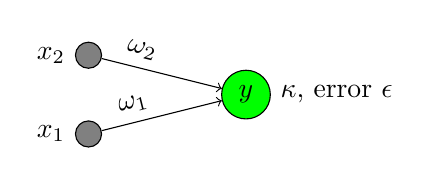
\begin{tikzpicture}
    [   cnode/.style={draw=black,fill=#1,minimum width=3mm,circle},
    ]
        \node[cnode=green,label=0:{$\kappa$, error $\epsilon$}] (s) at (2,-1.5) {$y$};
        \foreach \x in {1,...,2}
        {   \pgfmathparse{\x}
            \node[cnode=gray,label=180:$x_{\pgfmathresult}$] (x-\x) at (0,\x-3) {};
            \draw[->] (x-\x) -- node[above,sloped,pos=0.3] {$\omega_{\pgfmathresult}$} (s);
        }
  \end{tikzpicture}
\end{align*}
and keeping in mind that $\kappa$ is $\sigma(S) = \frac{1}{1+e^{-S}} = \frac{1}{1+e^{-\sum_{i=1}^n w_ix_i}}$ then the error can be expressed as 
$$ \epsilon = (\lambda - \kappa)^2  =  (\lambda - \sigma(S))^2$$ 
or in our example  
$$ \epsilon = \Big(\lambda - \frac{1}{1+e^{-w_1x_1-w_2x_2}}\Big)^2$$
Using gradient descent, minimizing $\epsilon$ with respect to node $x_i$ requires us to change $w_i$ by the negative of its gradient. This gradient is 

\begin{align}
  \frac{\partial MSE}{\partial w_i} = \frac{\partial(\lambda - \sigma(S))^2}{\partial w_i}  = \frac{\partial\sigma(S)}{\partial w_i}2(\lambda - \sigma(S))
  \label{eq:gradient_descent_on_sigma}
\end{align}

because $\sigma(S)$ is the only function of $w_i$. This is where having an activation function that can be easily differentiated is advantageous. For the sigma function, the derivative evaluates to
\begin{align}
\label{eq:sigma_derivative}
\sigma(S)\prime &=  \frac{\partial }{\partial S}{\frac{1}{1+e^{-S}}} \\
&= \frac{e^{-S}}{\Big({1+e^{-S}}\Big)^2} \\
&= \frac{1 + e^{-S} - 1}{\Big({1+e^{-S}}\Big)^2} \\
&= \frac{1 + e^{-S}}{\Big({1+e^{-S}}\Big)^2} - \frac{1}{\Big({1+e^{-S}}\Big)^2} \\
&= \frac{1}{{1+e^{-S}}} - \Big(\frac{1}{{1+e^{-S}}}\Big)^2 \\
&= \sigma(S) - \sigma(S)^2 \\
&= \sigma(S) * (1-\sigma(S)).
\label{eq:sigma_derivative}
\end{align}
the last step is carried for notational simplicity. Combining equations \ref{eq:gradient_descent_on_sigma} and \ref{eq:sigma_derivative}, we find that the weight of the $i$th node $w_i$ must be changed by the negative of the gradient

\begin{align*}
  2\sigma(S)^\prime(\lambda - \sigma(S))
\end{align*}
which leads to a weight update rule of 
\begin{align}
  w_{i_{t+1}} = w_{i_t} - 2\sigma(S)^\prime(\lambda - \sigma(S))
  \label{eq:update_rule_for_sigma}
\end{align}

In this way, the error that is produced at the top layer, where the final classification decision is contrasted with the desired decision, trickles down to all lower layers, with each node changing its weights according to the error of the upper node. Back propagation is worked on out example above in Figure \ref{fig:back_propagation}.


\begin{figure}[!h]
  \begin{subfigure}{0.45\linewidth}
    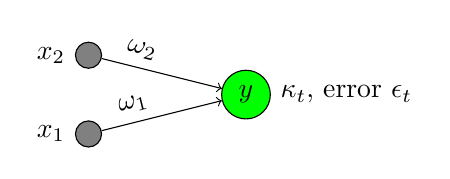
\begin{tikzpicture}
      [   cnode/.style={draw=black,fill=#1,minimum width=3mm,circle},
      ]
          \node[cnode=green,label=0:{$\kappa_t$, error $\epsilon_t$}] (s) at (2,-1.5) {$y$};
          \foreach \x in {1,...,2}
          {   \pgfmathparse{\x}
              \node[cnode=gray,label=180:$x_{\pgfmathresult}$] (x-\x) at (0,\x-3) {};
              \draw[->] (x-\x) -- node[above,sloped,pos=0.3] {$\omega_{\pgfmathresult}$} (s);
          }
    \end{tikzpicture}
    \caption{at time $t$}
  \end{subfigure}
  \begin{subfigure}{0.45\linewidth}
    \begin{tikzpicture}
      [   cnode/.style={draw=black,fill=#1,minimum width=3mm,circle},
      ]
          \node[cnode=green,label=0:{$\kappa_{t+1}$, error $\epsilon_{t+1}$}] (s) at (5,3) {$y$};
          \foreach \x in {1,...,2}
          {   \pgfmathparse{\x}
              % z=\x-1
              \node[cnode=gray,label=180:$x_{\pgfmathresult}$] (x-\x) at ($(0,0)+ (0, {\x*2}) $) {};
              \draw[->] (x-\x) -- node[above,sloped,pos=0.3] {$\omega_{\pgfmathresult} - 2\omega_{\pgfmathresult}x_{\pgfmathresult}(\lambda - \kappa_t)$} (s);
          }
    \end{tikzpicture}
    \caption{at time $t+1$}
  \end{subfigure}
  \caption{Back propagation works by minimizing the error function using gradient descent. In this case, the error function is the MSE, and its partial derivative with respect to each weight from the $i$th node in the previous layer is $2w_ix_i(\lambda - \kappa_t$ where $\lambda$ is the desired outcome and $\kappa_t$ is the predicted outcome at iteration $t$. In each iteration, applying gradient descent results in a move towards the opposite of the gradient, meaning partial derivative of the error with respect to that weight is negated from the weight (right). This method is guaranteed to converge, however slowly, over well defined continuous activation functions, an example of which is the sigmoid function (Fig. \ref{fig:activation_functions}).}
  \label{fig:back_propagation}
\end{figure}

Some of these networks, if constructed properly, can solve linearly inseparable problems.
%TODO: Could talk about how to find if a datset is linearly separable. Could we use Perceptrons to do it?















\subsubsection{Decision Trees}
\label{sec:decision_trees}
A completely different approach to label classification is that of using decision trees to find the features that are most likely to hint at a correct approach towards finding a solution. For example, consider a problem where both the input and the output of the data is categorical. One such dataset is the swimming pool and weather dataset, in which each data point is a weather description of a day and whether or not the tennis court was open on that day (Table \ref{table:categorial_examples_weather}). In this dataset there are several weather-related features such as \textit{Outlook, Temperature, Humidity,} and \textit{Wind}. The \textit{Outlook} feature could contain categories such as sunny, overcast, or rainy; the \textit{Temperature} feature could include categories such as hot or cold; the wind category could include Strong or Weak. All these features contain values from finite set of possibilities. 

\begin{table}
\begin{center}
     \begin{tabular}{||c c c c c c||} 
    \hline
     Day & Outlook & Temperature & Humidity & Wind & Play \\ [0.5ex] 
    \hline\hline
     D1 & Sunny & Hot & High & Weak  & No\\ 
    \hline
     D2 & Sunny & Hot & High & Strong  & No\\ 
    \hline
     D3 & Overcast & Hot & High & Weak  & Yes\\ 
    \hline
     D4 & Rainy & Mild & High & Weak  & Yes\\ 
    \hline
     D5 & Rainy & Cool & Normal & Weak  & Yes\\ 
    \hline
     D6 & Rainy & Cool & Normal & Strong  & No\\ 
    \hline
     D7 & Overcast & Cool & Normal & Strong  & Yes\\ 
    \hline
     D8 & Sunny & Mild & High & Weak  & No\\ 
    \hline
     D9 & Sunny & Cool & Normal & Weak  & Yes\\ 
    \hline
     D10 & Rainy & Mild & Normal & Weak  & Yes\\ 
    \hline
     D11 & Sunny & Mild & Normal & Strong  & Yes\\ 
    \hline
     D12 & Overcast & Mild & High & Strong  & Yes\\ 
    \hline
     D13 & Overcast & Hot & Normal & Weak  & Yes\\ 
    \hline
     D14 & Rainy & Mild & High & Strong & No\\  [1ex]
    \hline
  \end{tabular}
\end{center}
\caption{Weather and Tennis court dataset example \cite{mitchell1997machine}. All features are categorical, meaning the values of the features are from a finite, relatively small set of possibilities. The values can not be numerically represented in a formula or compared, nor do they represent values on a range.}
\label{table:categorial_examples_weather}
\end{table}

Through a simple observation at the table, we can perhaps device our own conditions for when the tennis court is open.
\begin{align*}
    \textrm{If outlook}&=\textrm{sunny } \wedge \textrm{ humidity = high, then Yes} \\
    \textrm{If outlook}&= \textrm{rainy } \wedge \textrm{ wind = Strong , then Yes} \\
    \textrm{Otherwise, No}
\end{align*}

Although this might be a good rule to follow, it might not generalize well to the rest of the dataset, and inspecting the entire dataset by eye becomes unfeasible beyond $~20$ data points. This is where the decision tree algorithm comes in, offering an automated method of finding such rules by which we can separate data points into \textit{Yes} and \textit{No} piles. In the simplest decision tree algorithm algorithm, the data points are iteratively separated by the feature that splits the data most evenly (or produces the most homogeneity within a feature split). For example, if we were to take the \textit{Wind} feature and split the Strong and Weak wind conditions into two piles, and observe how mixed or 'pure' the piles are, we would get a sense of how well the \textit{Wind} feature can split up our decision (Fig \ref{fig:split_on_wind}).

\begin{figure}
  \centering
    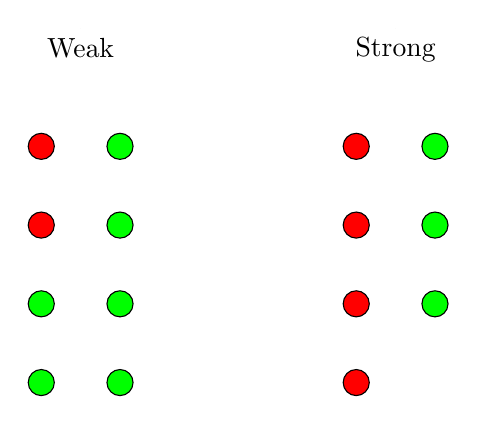
\begin{tikzpicture}
      [   cnode/.style={draw=black,fill=#1,minimum width=3mm,circle},
      ]
          \filldraw[black] (0.5, 1.5) circle (0pt) node[anchor=north] {Weak};
          \node[cnode=red] (s) at (0,0) {};
          \node[cnode=red] (s) at (0,-1) {};
          \node[cnode=green] (s) at (0,-2) {};
          \node[cnode=green] (s) at (0,-3) {};
          \node[cnode=green] (s) at (1,0) {};
          \node[cnode=green] (s) at (1,-1) {};
          \node[cnode=green] (s) at (1,-2) {};
          \node[cnode=green] (s) at (1,-3) {};

          \filldraw[black] (4.5, 1.5) circle (0pt) node[anchor=north] {Strong};
          \node[cnode=red] (s) at (4,0) {};
          \node[cnode=red] (s) at (4,-1) {};
          \node[cnode=red] (s) at (4,-2) {};
          \node[cnode=red] (s) at (4,-3) {};
          \node[cnode=green] (s) at (5,0) {};
          \node[cnode=green] (s) at (5,-1) {};
          \node[cnode=green] (s) at (5,-2) {};
    \end{tikzpicture}
    \caption{The decisions to play or not play tennis when the decision is split on wind conditions. Red balls represent No and green balls represent Yes. As we can tell from this graph, splitting on the Wind feature does not provide a homogeneous set (both sides of the split are not purely green or purely red). This means that we can't conclude that whenever the wind is strong tennis can not be played, vise versa. However, It seems that the split caused us to see a relationship between wind conditions and playing tennis, since when the wind was weak most decisions were to play tennis, while when it was wind most decisions were not to play tennis.}
    \label{fig:split_on_wind}
\end{figure}

This idea of purity or homogeneity is represented in the mathematical formula for entropy (taken from the Information Theory field) as follow

\begin{align}
Entropy = \sum_{i=1}^n p_i log_n(p_i)
\end{align}
where $n$ is the number of decisions possible and $p_i$ is the fraction of the decisions that were in the $i$th decision. This definition can be used to calculate the entropy in each of our splits. In our \textit{Wind} feature split example, we can measure the entropy in our Strong and Weak split. In each split our decision possibilities were two (Yes or No); our Strong split had 0.57 fraction No and 0.43 Yes; our Weak split had 0.25 fraction No and 0.75 fraction Yes. So the entropy calculation for the Strong split becomes

$$ - \Big(  0.57*log_2(0.57) + 0.43*log_2(0.43)  \Big) = 0.985$$
and for the Weak split the entropy is
$$ - \Big(  0.25*log_2(.25) + .75*log_2(.75)   \Big) = 0.811 \text{ .}$$

Figure \ref{fig:entropy_two_decisions} provides some intuition as to what entropy measures. Using this metric, we can devise an algorithm to iteratively pick the feature that that contains the least entropy when splitting the data upon. However, a more concrete way of using Entropy is measuring \textit{Information Gain} on each split. Information gain is a measure of how much entropy is lost through a transition. The equation that describes information gain is

\begin{align}
\textit{Information Gain} = Entropy(S) - \sum_{v\in Values(F)} \frac{|T_v|}{|T|}Entropy(T_v)
\end{align}
where F is the feature we are splitting on, $|T_v|$ is the number of decisions with split value $v$, $|T|$ the number of total decisions, and $Entropy(T_v)$ is the measure of entropy on the decisions with split value $v$. In our wind example, the entropy of the original system (without any splitting on any feature) is $-\big(\frac{5}{14}*log_2(5/14) + \frac{9}{14}*log_2(9/14) \big) =  0.94$. Since we had two splits on \textit{Wind}, let $v_1$ be the Strong split and $v_2$ be the Weak split then

\begin{align*}
  \textit{Information Gain(Wind)} &= Entropy(Original) - \frac{|T_{v_1}|}{|T|}Entropy(T_{v_1}) - \frac{|T_{v_2}|}{|T|}Entropy(T_{v_2}) \\
   &= 0.94 - \frac{6}{14}0.985 - \frac{8}{14}0.811 \\
   &= 0.054
\end{align*}

In this manner, we can measure the information gain on splitting on each available feature, and choose the feature that results in the highest information gain split. This would give us two to three bins, on which we iteratively carry out this process again choosing another feature and so on. A decision tree is the amalgamation of all these decisions, put in a concise diagram (Fig. \ref{fig:decision_tree_for_tennis}). This algorithm has the distinct advantage of being able to display its reasoning efficiently, a feat that some machine learning algorithms can not accomplish.

\begin{figure}
  \centering
  \includegraphics[width=0.7\linewidth]{figures/entropy_fig.pdf}
  \caption{The entropy of a system with two decisions each of which have a fraction $p_1$ and $p_2$ (fraction $p_2$ is not shown here because it is simply $1-p_1$). When the system has both fractions in equal proportions, it is perfectly heterogeneous, so it has the highest entropy measure of $1$. On the other end, when one fraction dominates the system, the entropy goes to $0$. In this way, entropy measures how "polluted" or pure a system is, giving a higher score to disorganized, polluted systems, and a lower score to homogeneous, pure systems.}
  \label{fig:entropy_two_decisions}
\end{figure}

\begin{figure}
\centering
\includegraphics[width=0.7\linewidth]{figures/tennis_decision_tree_mitchel.png}
\caption{A decision tree that can be generated by iterating over the tennis-weather dataset using the information gain equation. This is taken from Michel's book on Machine Learning \cite{mitchell1997machine}.}
\label{fig:decision_tree_for_tennis}
\end{figure}



\subsubsection{Regression Prediction}
\label{sec:regression_supervised_learning}
For cases when the desired output of a function is a number on a meaningful range, label classification is not possible. This is because a supervised label classification problem deals with \textit{choosing} the best label out of a given set, and not generating a label out of the given data. This is where regression prediction comes into play. For functions whose output is a continuous range of numbers, one can not possibly assign a label to each possible output. And even if each output is assignable, there is rarely a dataset big enough to cover possible mappings to each such label.

For example, given an input set of ${1,2,3,4,5,6,7}$ and an output set ${1,4,9,14,25,36,49}$, a good---and almost any---supervised learning algorithm should approximate the function $f(x^2)$. However, such a function would have rely on regression learning, and not label classification. To show this, let's delve into a thinking exercise. Say we make a training set for the function $f(x) = x^2$ consisting of input that is all the integers from one to one million and output that is the square of all these input numbers. If we are to use label classification, then we would train the algorithm to map each number to its square label. The first problem arises on the first step of learning, especially in the Decision Tree technique. Because each input is looked at as a categorical input, an input of one (1) will be converted to a label. Since each data point has its own label, the information gain will be maximized and the entropy loss will be minimized when the input is split into one million branches on the first level of the tree. At that point, the function mapping is resolved by simply going through one level. However, this leads to the second problem, which arises when feeding in new test data that the classifier was not trained on. Because the classifier only has access to labels that it trained on, any number other than an integer from one to million will have to map to an already known label from the squares of the integers from one to one million. For example, an input of $1.76$ will map to either $1$ ($1^2=1$) or $4$ ($2^2 = 4$), meaning this incurs an accuracy cost. This cost might not be a big problem for the purposes of the algorithm, but the real problem arises when we try to predict the mapping of a number outside the range of our training dataset: numbers below 0 and those above one million. The nearest value for all numbers below 0 is $1$, so all the numbers below 0 will be mapped to the label of $0$, while all the numbers above one million will be mapped to the label of one million (Fig \ref{fig:decision_tree_regression_and_classification}).

\begin{figure}[!h]
  \centering
    \begin{subfigure}{0.49\textwidth}
        \centering
        \includegraphics[width=\linewidth]{figures/reg_tree.pdf}
        \caption{Regression Decision Tree}
    \end{subfigure}
    \begin{subfigure}{0.49\textwidth}
        \centering
        \includegraphics[width=\linewidth]{figures/reg_tree_plot.pdf}
        \caption{Regression Decision Test Results}
    \end{subfigure}
  \caption{A Decision Tree trained on a dataset of simple square functions, where the inputs were numbers from 0 to 10 and output is the square of each number. The tree shows a jagged approximation of the square function between 0 and 10, which indicates some level of learning. However, the tree shows very poor generalization outside the learning range. When tested on input that is below 0, the tree matches to the closest label in the decision boundary, which is "0". A similar decision is made for input that is greater than 10, where the trees matches all numbers greater than 10 to the label of 10 ("100").}
  \label{fig:decision_tree_regression_and_classification}
\end{figure}

From this small experiment, the need for a different approach to supervised learning is obvious. Such a technique would need to generalize the mapping not to categorical labels and their limited space, but to an unlimited range of numbers. This method would solve a more conventional mathematical problem of function approximation. Another way to think about the problem is curve fitting: given input and output sets, the curve of the approximated function should pass---or be proximal---the points given in the sets. The best fit for our function would be a curve that passes perfectly through all our data points. As the approximated curve moves further and further away from the given points, the distance between the points and the curve increases, which we can use as a measurement of error (Fig. \ref{fig:error_lines}). The sum of this error can be expressed as

\begin{figure}[!h]
  \centering
  \includegraphics[width=0.7\linewidth]{figures/error_lines.pdf}
  \caption{Different lines of fit and their errors (dashed and dotted lines) with respect to the noisy input data. Because $g(x)$ and $h(x)$ have larger error lines than $f(x)$, $f(x)$ is the best fit for the data out of the three drawn lines. Note that for $f(x)$, the negative and positive errors cancel out, leading to a sum of error of $-21$. This is allayed by summing the square of the error instead, which results in an equation that can be minimized to $176$.}
  \label{fig:error_lines}
\end{figure}

\begin{align*}
  Error &= \sum_{i=1}^n (y_i-f(x_i)),
\end{align*}

where for the $i$th data point $y_i$ represents the actual $y$ value and $f(x_i)$ represents the approximation of the regression line at $x_i$. Minimizing this error term ensures that our resulting function is the closes line fit to our data points. However, notice that in our error function, positive and negative errors will cancel out, leading to the assumption that "two wrongs make a right". To avoid this, we can either take the absolute value of the error, or the square. For mathematical convenience, the squared error is preferred. This results in the method of Least Squared Error (LSE) as given by

\begin{align}
\label{eq:least_square}
LSE &= \sum_{i=0}^n (y_i-f(x_i))^2  = \sum_{i=0}^n (y_i- b_0 - b_1x_i)^2
\end{align}

From this equation it can be shown that 

\begin{align}
b_1 &= \frac{\sum_{i=1}^n y_ix_i - \frac{\sum_{i=1}^n y_i \sum_{i=1}^n x_i}{n}}{\sum_{i=1}^n x_i^2 - \frac{\Big(\sum_{i=1}^n x_i \Big)^2}{n}}
\end{align}

and 
$$ b_0 = \bar y - b_1 \bar x $$

where $\bar y$ and $\bar x$ are the respective means of all $y$ and $x$ values \cite{Finney1996}. This formula guarantees a line of best fit that minimizes squared errors for linear data points. For cases when the data points do not display a linear behavior, they can be transformed into a space where they become more linear, linear regression applied, and the regression functions transformed back into the original space (Fig \ref{fig:log_regression}).

\begin{figure}[!h]
  \centering
    \begin{subfigure}{0.32\textwidth}
        \centering
        \includegraphics[width=\linewidth]{figures/regression_log_example_1.pdf}
    \end{subfigure}
  \begin{subfigure}{.32\textwidth}
        \centering
        \includegraphics[width=\linewidth]{figures/regression_log_example_2.pdf}
    \end{subfigure}
    \begin{subfigure}{0.32\textwidth}
        \centering
        \includegraphics[width=\linewidth]{figures/regression_log_example_3.pdf}
    \end{subfigure}
  \caption{Finding line of least squared error for data with an exponential trend. First, the data points (Left) are transformed to their logs (Center). Then a line of best fit is found through linear regression (Center). The line is then transformed back to the original space by applying the exponential function (Right).}
  \label{fig:log_regression}
\end{figure}

Using this regression model for out previous example in Figure \ref{fig:decision_tree_regression_and_classification}, we are able to attain more realistic learning through a model that extrapolates more correctly to unseen numeric data (Fig. \ref{fig:regression_on_square_function})

\begin{figure}[!h]
  \centering
    \includegraphics[width=0.7\linewidth]{figures/reg_ridge_plot.pdf}
  \caption{Using a non-linear regression model for the same data set used on in Figure \ref{fig:decision_tree_regression_and_classification}, we are able to build a model that correctly extrapolates to unseen numeric data. Since this is one of the requirements for problems with outputs being continuous numbers, thsi model is highly valuable for prediction in such output spaces.}
  \label{fig:regression_on_square_function}
\end{figure}
%We might be able to include support vector machines.